\documentclass[aspectratio=169]{beamer}

\usetheme{default}
\usecolortheme{dove}

\setbeamertemplate{navigation symbols}{}
\setbeamertemplate{footline}{%
  \hfill{\large\insertframenumber\,/\,\inserttotalframenumber}\hspace{0.8em}\vspace{0.5em}%
}

\definecolor{popblue}{RGB}{52, 101, 164}
\definecolor{sampred}{RGB}{204, 0, 0}
\definecolor{paramgreen}{RGB}{0, 140, 70}
\definecolor{warnred}{RGB}{180, 40, 40}
\definecolor{orange1}{RGB}{220, 120, 0}
\definecolor{violet1}{RGB}{120, 50, 160}
\definecolor{lightbg}{RGB}{245, 245, 250}

\setbeamercolor{frametitle}{fg=popblue}
\setbeamercolor{title}{fg=popblue}

\usepackage{pgfplots}
\usepackage{tikz}
\usetikzlibrary{shapes, arrows.meta, positioning, calc, decorations.pathreplacing, patterns}
\pgfplotsset{compat=1.18}
\usepackage{amsmath, amssymb}
\usepackage{fontenc}

\title{Lecture 7: Confidence Intervals}
\subtitle{Sampling Distributions $\cdot$ Standard Errors $\cdot$ Interval Estimation}
\date{}

\begin{document}

% ============================================================
\begin{frame}
\titlepage
\end{frame}

% ============================================================
\begin{frame}
\frametitle{Previously, on Lectures 5 \& 6\ldots}

\begin{center}
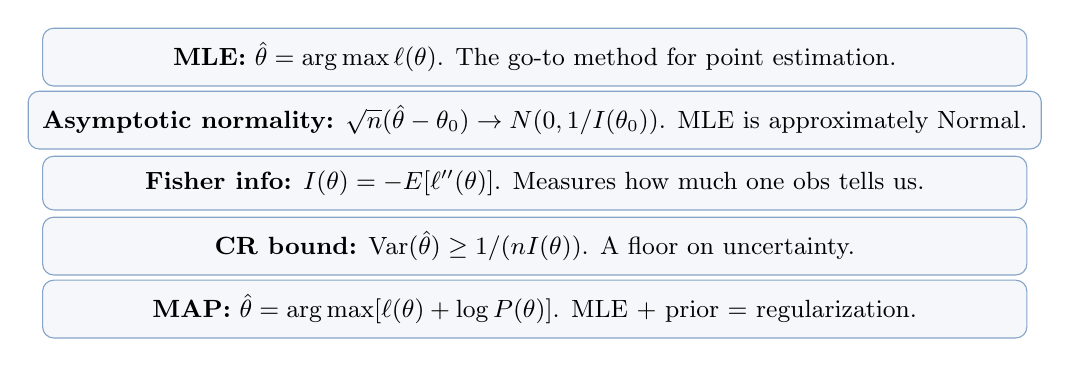
\begin{tikzpicture}[
  sbox/.style={draw=popblue!60, fill=popblue!5, rounded corners=4pt, minimum width=12.5cm, minimum height=0.5cm, align=left, inner sep=5pt, font=\small}
]
  \node[sbox] at (0, 2.0) {\textbf{MLE:} $\hat\theta = \arg\max \ell(\theta)$. The go-to method for point estimation.};
  \node[sbox] at (0, 1.2) {\textbf{Asymptotic normality:} $\sqrt{n}(\hat\theta - \theta_0) \to N(0, 1/I(\theta_0))$. MLE is approximately Normal.};
  \node[sbox] at (0, 0.4) {\textbf{Fisher info:} $I(\theta) = -E[\ell''(\theta)]$. Measures how much one obs tells us.};
  \node[sbox] at (0, -0.4) {\textbf{CR bound:} $\text{Var}(\hat\theta) \geq 1/(nI(\theta))$. A floor on uncertainty.};
  \node[sbox] at (0, -1.2) {\textbf{MAP:} $\hat\theta = \arg\max[\ell(\theta) + \log P(\theta)]$. MLE + prior = regularization.};
\end{tikzpicture}
\end{center}

\vspace{0.3cm}
\begin{center}
{\large\textbf{Today:}} A point estimate is just a number. How \textbf{uncertain} is it?\\[4pt]
``52\% support candidate A'' means nothing without $\pm$ something.
\end{center}
\end{frame}

% ============================================================
\section{Sampling Distributions}

\begin{frame}
\begin{center}
  \vspace{2cm}
  {\Huge\bfseries\textcolor{popblue}{Sampling Distributions}}

  \vspace{0.8cm}
  {\large Your estimator is a random variable}
\end{center}
\end{frame}

\begin{frame}
\frametitle{The Key Idea: $\hat\theta$ Is Random}

\begin{center}
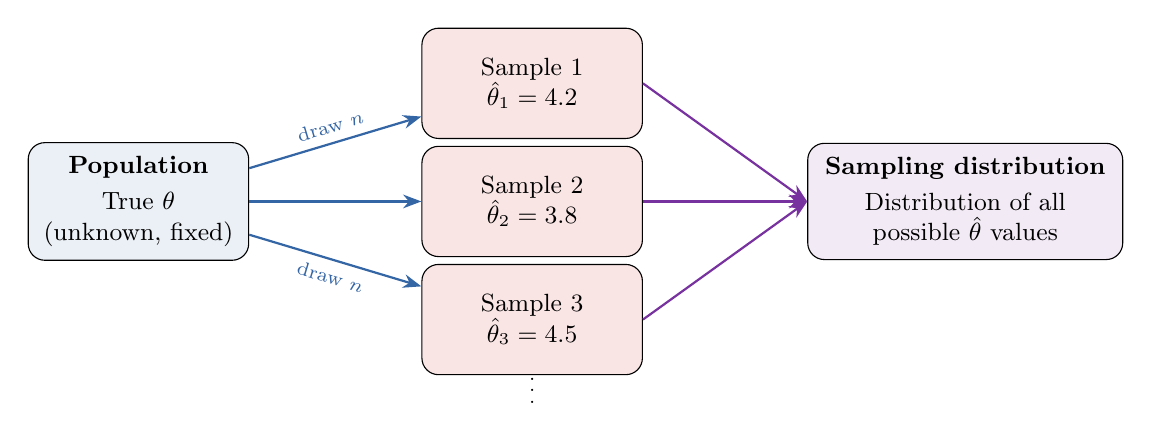
\begin{tikzpicture}[
  box/.style={draw, rounded corners=6pt, minimum width=2.8cm, minimum height=1.4cm, align=center, font=\small, inner sep=5pt}
]
  % Population
  \node[box, fill=popblue!10] (pop) at (-5, 0) {\textbf{Population}\\[2pt]True $\theta$\\(unknown, fixed)};

  % Samples
  \node[box, fill=sampred!10] (s1) at (0, 1.5) {Sample 1\\$\hat\theta_1 = 4.2$};
  \node[box, fill=sampred!10] (s2) at (0, 0) {Sample 2\\$\hat\theta_2 = 3.8$};
  \node[box, fill=sampred!10] (s3) at (0, -1.5) {Sample 3\\$\hat\theta_3 = 4.5$};

  \draw[-{Stealth}, thick, popblue] (pop) -- (s1) node[midway, above, font=\scriptsize, sloped] {draw $n$};
  \draw[-{Stealth}, thick, popblue] (pop) -- (s2);
  \draw[-{Stealth}, thick, popblue] (pop) -- (s3) node[midway, below, font=\scriptsize, sloped] {draw $n$};

  % Histogram
  \node[box, fill=violet1!10, minimum width=4cm] (hist) at (5.5, 0) {\textbf{Sampling distribution}\\[2pt]Distribution of all\\possible $\hat\theta$ values};

  \draw[-{Stealth}, thick, violet1] (s1.east) -- (hist.west);
  \draw[-{Stealth}, thick, violet1] (s2.east) -- (hist.west);
  \draw[-{Stealth}, thick, violet1] (s3.east) -- (hist.west);

  \node[font=\scriptsize] at (0, -2.3) {$\vdots$};
\end{tikzpicture}
\end{center}

\pause
\vspace{0.2cm}
\centering\small
Each sample gives a \textbf{different} estimate. The \textbf{sampling distribution} describes this variability.
\end{frame}

\begin{frame}
\frametitle{The Sampling Distribution of $\bar{X}$}

\small
If $X_1, \ldots, X_n \overset{\text{iid}}{\sim} (\mu, \sigma^2)$, what is the distribution of $\bar{X} = \frac{1}{n}\sum X_i$?

\pause
\vspace{0.2cm}
\begin{center}
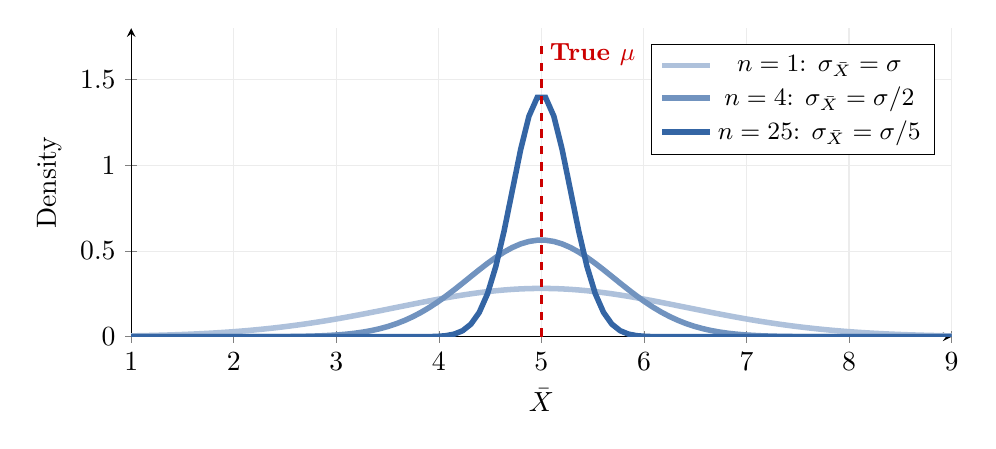
\begin{tikzpicture}
  \begin{axis}[
    width=12cm, height=5.5cm,
    xlabel={$\bar{X}$},
    ylabel={Density},
    xmin=1, xmax=9,
    ymin=0, ymax=1.8,
    axis lines=left,
    legend style={at={(0.98,0.95)}, anchor=north east, font=\small},
    grid=major, grid style={gray!15},
    every axis plot/.append style={line width=2pt, samples=100}
  ]
    % n=1: wide
    \addplot[popblue!40, domain=1:9] {exp(-(x-5)^2/(2*2))/(sqrt(2*pi*2))};
    \addlegendentry{$n=1$: $\sigma_{\bar{X}} = \sigma$}

    % n=4: medium
    \addplot[popblue!70, domain=1:9] {exp(-(x-5)^2/(2*0.5))/(sqrt(2*pi*0.5))};
    \addlegendentry{$n=4$: $\sigma_{\bar{X}} = \sigma/2$}

    % n=25: narrow
    \addplot[popblue, domain=1:9] {exp(-(x-5)^2/(2*0.08))/(sqrt(2*pi*0.08))};
    \addlegendentry{$n=25$: $\sigma_{\bar{X}} = \sigma/5$}

    % True value
    \draw[dashed, sampred, thick] (axis cs:5, 0) -- (axis cs:5, 1.7);
    \node[font=\small\bfseries, sampred] at (axis cs:5.5, 1.65) {True $\mu$};
  \end{axis}
\end{tikzpicture}
\end{center}

\pause
\vspace{-0.1cm}
\centering
$\bar{X} \sim N\!\left(\mu, \;\frac{\sigma^2}{n}\right)$ \quad (exactly if Normal; approximately by CLT otherwise)
\end{frame}

\begin{frame}
\frametitle{The $\sqrt{n}$ Law}

\begin{center}
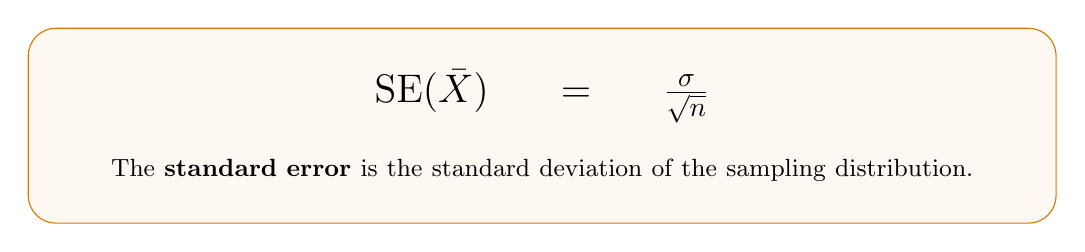
\begin{tikzpicture}
  \node[draw=orange1, fill=orange1!5, rounded corners=10pt, text width=12cm, align=center, inner sep=15pt] {
    {\Large
    $\text{SE}(\bar{X}) = \frac{\sigma}{\sqrt{n}}$
    }\\[12pt]
    \small The \textbf{standard error} is the standard deviation of the sampling distribution.
  };
\end{tikzpicture}
\end{center}

\pause
\vspace{0.3cm}
\begin{center}
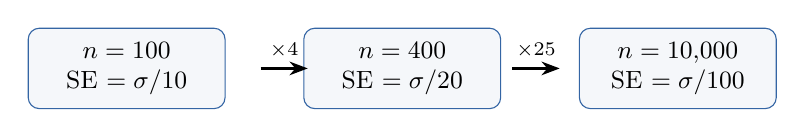
\begin{tikzpicture}[
  nbox/.style={draw=popblue, fill=popblue!5, rounded corners=4pt, minimum width=2.5cm, minimum height=1cm, align=center, font=\small, inner sep=5pt}
]
  \node[nbox] at (-5, 0) {$n = 100$\\SE $= \sigma/10$};
  \node[nbox] at (-1.5, 0) {$n = 400$\\SE $= \sigma/20$};
  \node[nbox] at (2, 0) {$n = 10{,}000$\\SE $= \sigma/100$};

  \draw[-{Stealth}, thick] (-3.3, 0) -- (-2.7, 0) node[midway, above, font=\scriptsize] {$\times 4$};
  \draw[-{Stealth}, thick] (-0.1, 0) -- (0.5, 0) node[midway, above, font=\scriptsize] {$\times 25$};
\end{tikzpicture}
\end{center}

\pause
\vspace{0.2cm}
\begin{center}
\fcolorbox{warnred}{warnred!5}{\parbox{10cm}{\centering\small
  To \textbf{halve} the standard error, you must \textbf{quadruple} the sample size.\\[2pt]
  Precision is expensive! Diminishing returns from more data.
}}
\end{center}
\end{frame}

\begin{frame}
\frametitle{Standard Error: Known vs Estimated}

\small
\begin{center}
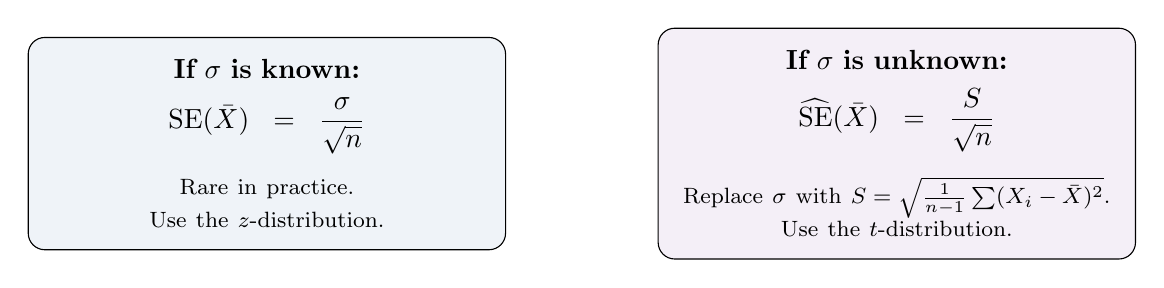
\begin{tikzpicture}[
  cbox/.style={draw, rounded corners=6pt, minimum height=2.5cm, text width=5.5cm, align=center, inner sep=8pt}
]
  \node[cbox, fill=popblue!8] at (-4, 0) {
    \textbf{If $\sigma$ is known:}\\[6pt]
    $\text{SE}(\bar{X}) = \dfrac{\sigma}{\sqrt{n}}$\\[8pt]
    \footnotesize Rare in practice.\\
    Use the $z$-distribution.
  };

  \pause
  \node[cbox, fill=violet1!8] at (4, 0) {
    \textbf{If $\sigma$ is unknown:}\\[6pt]
    $\widehat{\text{SE}}(\bar{X}) = \dfrac{S}{\sqrt{n}}$\\[8pt]
    \footnotesize Replace $\sigma$ with $S = \sqrt{\frac{1}{n-1}\sum(X_i - \bar{X})^2}$.\\
    Use the $t$-distribution.
  };
\end{tikzpicture}
\end{center}

\pause
\vspace{0.3cm}
\begin{center}
\fcolorbox{popblue}{popblue!5}{\parbox{10cm}{\centering\small
  \textbf{General pattern for any MLE} (from Lecture~5):\\[3pt]
  $\widehat{\text{SE}}(\hat\theta_{\text{MLE}}) = \frac{1}{\sqrt{n \cdot I(\hat\theta)}}$
  \quad --- plug in $\hat\theta$ for $\theta$ in the Fisher information.
}}
\end{center}
\end{frame}

% ============================================================
\section{Confidence Intervals}

\begin{frame}
\begin{center}
  \vspace{2cm}
  {\Huge\bfseries\textcolor{popblue}{Confidence Intervals}}

  \vspace{0.8cm}
  {\large From point estimate to interval estimate}
\end{center}
\end{frame}

\begin{frame}
\frametitle{What Is a Confidence Interval?}

\begin{center}
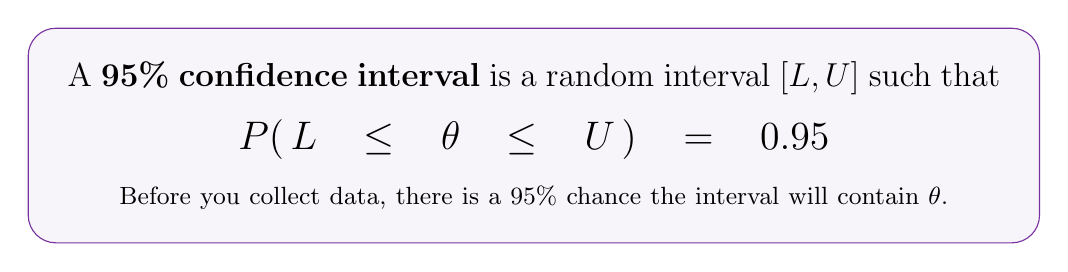
\begin{tikzpicture}
  \node[draw=violet1, fill=violet1!5, rounded corners=10pt, text width=12cm, align=center, inner sep=12pt] {
    {\large A \textbf{95\% confidence interval} is a random interval $[L, U]$ such that}\\[8pt]
    {\Large $P(\,L \leq \theta \leq U\,) = 0.95$}\\[8pt]
    \small Before you collect data, there is a 95\% chance the interval will contain $\theta$.
  };
\end{tikzpicture}
\end{center}

\pause
\vspace{0.1cm}
\begin{center}
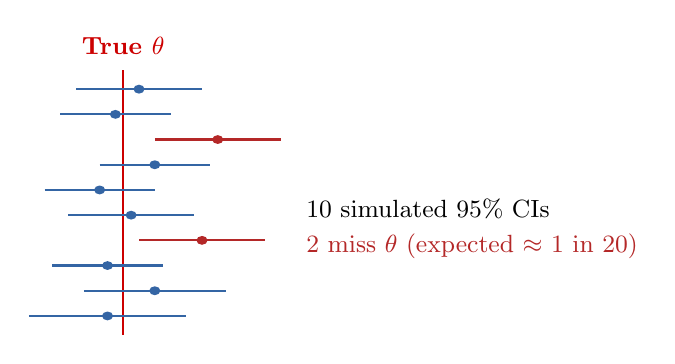
\begin{tikzpicture}[yscale=0.8]
  % True theta line
  \draw[thick, sampred] (0, 0) -- (0, 4.2);
  \node[font=\small\bfseries, sampred, above] at (0, 4.3) {True $\theta$};

  % CI lines
  \foreach \y/\l/\r/\col in {0.3/-1.2/0.8/popblue, 0.7/-0.5/1.3/popblue, 1.1/-0.9/0.5/popblue, 1.5/0.2/1.8/warnred, 1.9/-0.7/0.9/popblue, 2.3/-1.0/0.4/popblue, 2.7/-0.3/1.1/popblue, 3.1/0.4/2.0/warnred, 3.5/-0.8/0.6/popblue, 3.9/-0.6/1.0/popblue} {
    \draw[thick, \col] (\l, \y) -- (\r, \y);
    \fill[\col] ({(\l+\r)/2}, \y) circle (2pt);
  }

  \node[font=\small, right] at (2.2, 2) {10 simulated 95\% CIs};
  \node[font=\small, warnred, right] at (2.2, 1.4) {2 miss $\theta$ (expected $\approx$ 1 in 20)};
\end{tikzpicture}
\end{center}
\end{frame}

\begin{frame}
\frametitle{Constructing the Wald CI}

\small
Since $\hat\theta$ is approximately Normal (by CLT or MLE asymptotics):
$\;\frac{\hat\theta - \theta}{\text{SE}(\hat\theta)} \approx N(0, 1)$

\pause
\vspace{0.05cm}
For a 95\% CI, we need $P(-1.96 \leq Z \leq 1.96) = 0.95$:

\pause
\vspace{0.05cm}
\begin{center}
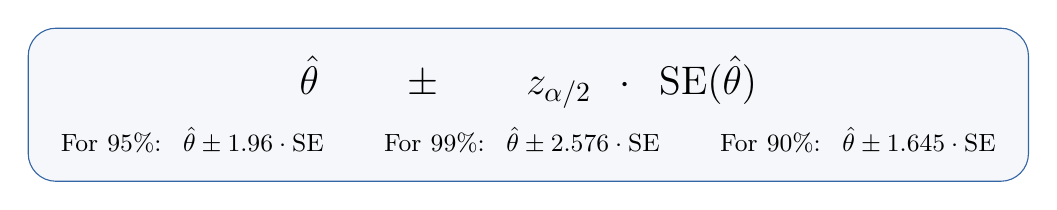
\begin{tikzpicture}
  \node[draw=popblue, fill=popblue!5, rounded corners=10pt, text width=12cm, align=center, inner sep=10pt] {
    {\Large $\hat\theta \;\pm\; z_{\alpha/2} \cdot \text{SE}(\hat\theta)$}\\[6pt]
    \small For 95\%: $\;\hat\theta \pm 1.96 \cdot \text{SE}$ \qquad
    For 99\%: $\;\hat\theta \pm 2.576 \cdot \text{SE}$ \qquad
    For 90\%: $\;\hat\theta \pm 1.645 \cdot \text{SE}$
  };
\end{tikzpicture}
\end{center}

\pause
\vspace{0.05cm}
\textbf{Recipe:}
\begin{enumerate}\setlength{\itemsep}{1pt}
  \item Compute the point estimate $\hat\theta$
  \item Compute (or estimate) the standard error $\text{SE}(\hat\theta)$
  \item Choose the confidence level $\Rightarrow$ look up $z_{\alpha/2}$
  \item Report: $\hat\theta \pm z_{\alpha/2} \cdot \text{SE}$
\end{enumerate}
\end{frame}

\begin{frame}
\frametitle{Example: CI for the Mean}

\small
\textbf{Setup:} $n = 36$ lightbulbs tested. $\;\bar{X} = 1{,}200$ hours, $\;S = 120$ hours.

\pause
\vspace{0.15cm}
\textbf{Step 1:} Point estimate: $\hat\mu = \bar{X} = 1{,}200$.

\pause
\textbf{Step 2:} Standard error: $\widehat{\text{SE}} = S / \sqrt{n} = 120/\sqrt{36} = 20$.

\pause
\textbf{Step 3:} For 95\%: $z_{0.025} = 1.96$.

\pause
\textbf{Step 4:}
$$\bar{X} \pm 1.96 \cdot \text{SE} = 1{,}200 \pm 1.96 \times 20 = 1{,}200 \pm 39.2$$

\vspace{0.1cm}
\begin{center}
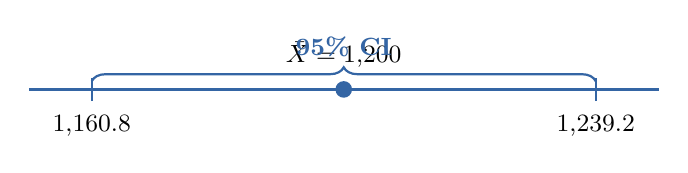
\begin{tikzpicture}
  \draw[thick, popblue] (-4, 0) -- (4, 0);
  \fill[popblue] (0, 0) circle (3pt);
  \node[font=\small, above] at (0, 0.15) {$\bar{X} = 1{,}200$};

  \draw[thick, popblue] (-3.2, -0.15) -- (-3.2, 0.15);
  \draw[thick, popblue] (3.2, -0.15) -- (3.2, 0.15);
  \node[font=\small, below] at (-3.2, -0.2) {1{,}160.8};
  \node[font=\small, below] at (3.2, -0.2) {1{,}239.2};

  \draw[thick, popblue, decorate, decoration={brace, amplitude=5pt, raise=3pt}] (-3.2, 0) -- (3.2, 0) node[midway, above, yshift=8pt, font=\small\bfseries] {95\% CI};
\end{tikzpicture}
\end{center}

\vspace{0.1cm}
\centering\small
``We are 95\% confident that the true mean lifetime is between 1{,}161 and 1{,}239 hours.''
\end{frame}

\begin{frame}
\frametitle{What 95\% Confidence \textbf{Really} Means}

\begin{center}
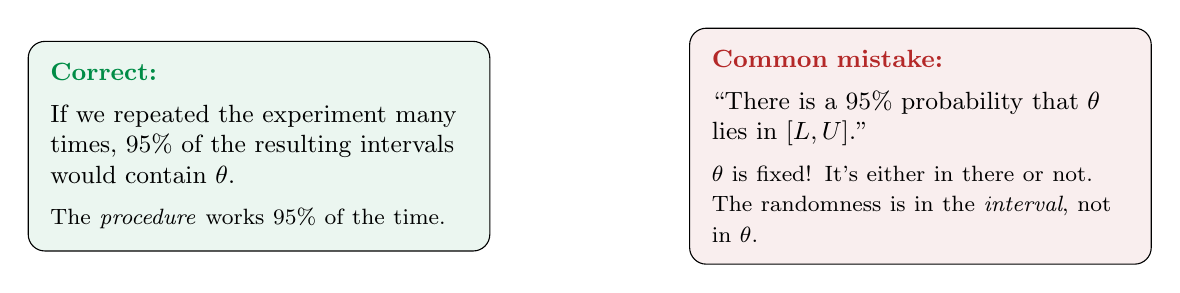
\begin{tikzpicture}[
  cbox/.style={draw, rounded corners=6pt, minimum height=2cm, text width=5.3cm, align=left, inner sep=8pt, font=\small}
]
  \node[cbox, fill=paramgreen!8] at (-4.2, 0) {
    \textbf{\textcolor{paramgreen}{Correct:}}\\[4pt]
    If we repeated the experiment many times, 95\% of the resulting intervals would contain $\theta$.\\[4pt]
    \footnotesize The \textit{procedure} works 95\% of the time.
  };

  \pause
  \node[cbox, fill=warnred!8] at (4.2, 0) {
    \textbf{\textcolor{warnred}{Common mistake:}}\\[4pt]
    ``There is a 95\% probability that $\theta$ lies in $[L, U]$.''\\[4pt]
    \footnotesize $\theta$ is fixed! It's either in there or not. The randomness is in the \textit{interval}, not in $\theta$.
  };
\end{tikzpicture}
\end{center}

\pause
\vspace{0.3cm}
\begin{center}
\fcolorbox{orange1}{orange1!5}{\parbox{10cm}{\centering\small
  \textbf{Analogy:} A 95\%-accurate archer hits the target 95\% of the time.\\
  After the arrow lands, it either hit or missed --- the probability is gone.\\[2pt]
  A CI is the arrow. Once computed, it either contains $\theta$ or it doesn't.
}}
\end{center}
\end{frame}

\begin{frame}
\frametitle{What Determines the Width?}

\begin{center}

\begin{tikzpicture}
  \node[draw=popblue, fill=popblue!5, rounded corners=8pt, text width=10cm, align=center, inner sep=12pt] {
    {\large Width $= 2 \cdot z_{\alpha/2} \cdot \dfrac{S}{\sqrt{n}}$}
  };
\end{tikzpicture}
\end{center}

\vspace{0.2cm}
\begin{center}
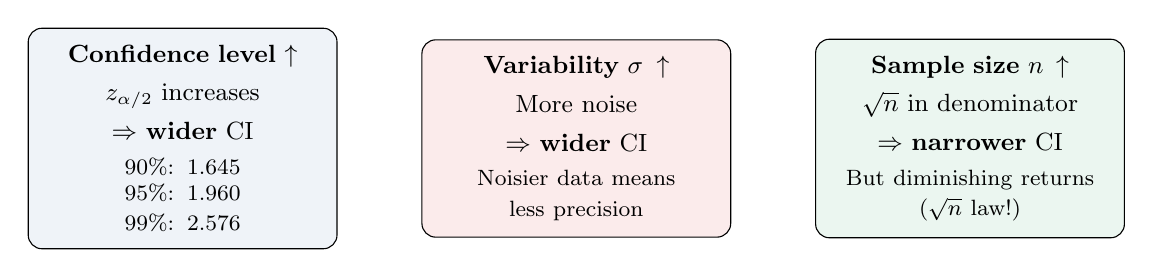
\begin{tikzpicture}[
  wbox/.style={draw, rounded corners=5pt, minimum height=1.8cm, text width=3.5cm, align=center, inner sep=6pt, font=\small}
]
  \node[wbox, fill=popblue!8] at (-5, 0) {
    \textbf{Confidence level $\uparrow$}\\[3pt]
    $z_{\alpha/2}$ increases\\[3pt]
    $\Rightarrow$ \textbf{wider} CI\\[3pt]
    \footnotesize 90\%: 1.645\\
    95\%: 1.960\\
    99\%: 2.576
  };

  \pause
  \node[wbox, fill=sampred!8] at (0, 0) {
    \textbf{Variability $\sigma \uparrow$}\\[3pt]
    More noise\\[3pt]
    $\Rightarrow$ \textbf{wider} CI\\[3pt]
    \footnotesize Noisier data means\\
    less precision
  };

  \pause
  \node[wbox, fill=paramgreen!8] at (5, 0) {
    \textbf{Sample size $n \uparrow$}\\[3pt]
    $\sqrt{n}$ in denominator\\[3pt]
    $\Rightarrow$ \textbf{narrower} CI\\[3pt]
    \footnotesize But diminishing returns\\
    ($\sqrt{n}$ law!)
  };
\end{tikzpicture}
\end{center}
\end{frame}

% ============================================================
\section{CIs for Proportions}

\begin{frame}
\begin{center}
  \vspace{2cm}
  {\Huge\bfseries\textcolor{popblue}{CIs for Proportions}}

  \vspace{0.8cm}
  {\large Polls, A/B tests, and defect rates}
\end{center}
\end{frame}

\begin{frame}
\frametitle{CI for a Proportion: The Wald Interval}

\small
\textbf{Setup:} $X_1, \ldots, X_n \sim \text{Bernoulli}(p)$. \; MLE: $\hat{p} = \bar{X} = k/n$.

\pause
\vspace{0.1cm}
\textbf{Variance:} $\text{Var}(\hat{p}) = p(1-p)/n$. \; Plug in $\hat{p}$:

$$\widehat{\text{SE}} = \sqrt{\frac{\hat{p}(1-\hat{p})}{n}}$$

\pause
\textbf{Wald 95\% CI:}
\begin{center}

\begin{tikzpicture}
  \node[draw=popblue, fill=popblue!5, rounded corners=8pt, text width=8cm, align=center, inner sep=10pt] {
    {\large $\hat{p} \;\pm\; 1.96\sqrt{\dfrac{\hat{p}(1-\hat{p})}{n}}$}
  };
\end{tikzpicture}
\end{center}

\pause
\vspace{0.15cm}
\textbf{Example:} Poll of $n = 1{,}000$ voters, $\hat{p} = 0.52$.
$$\text{SE} = \sqrt{\frac{0.52 \times 0.48}{1000}} = 0.0158 \qquad \text{CI: } 0.52 \pm 0.031 = [0.489,\; 0.551]$$

\centering\small The race is too close to call! The CI includes 0.5.
\end{frame}

\begin{frame}
\frametitle{When Wald Fails: Small $n$ or Extreme $\hat{p}$}

\small
\textbf{Problem:} $n = 20$, $k = 0$ (no successes). $\hat{p} = 0$.

\pause
\vspace{0.15cm}
Wald CI: $\;0 \pm 1.96\sqrt{0 \cdot 1/20} = [0,\; 0]$. \quad A \textbf{zero-width} interval!

\pause
\vspace{0.15cm}
\begin{center}
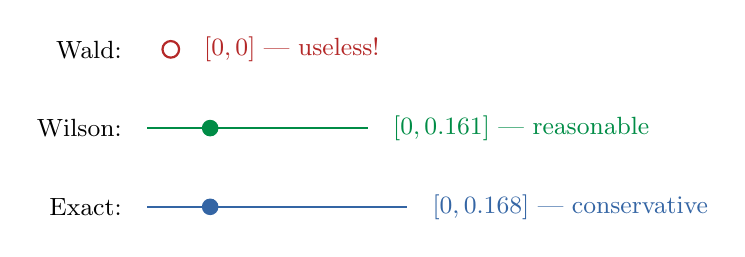
\begin{tikzpicture}
  % Wald: degenerate
  \draw[thick, warnred] (0, 1) circle (3pt);
  \node[font=\small, left] at (-0.5, 1) {Wald:};
  \node[font=\small, warnred, right] at (0.3, 1) {$[0, 0]$ --- useless!};

  % Wilson: sensible
  \draw[thick, paramgreen] (-0.3, 0) -- (2.5, 0);
  \fill[paramgreen] (0.5, 0) circle (3pt);
  \node[font=\small, left] at (-0.5, 0) {Wilson:};
  \node[font=\small, paramgreen, right] at (2.7, 0) {$[0, 0.161]$ --- reasonable};

  % Exact: Clopper-Pearson
  \draw[thick, popblue] (-0.3, -1) -- (3.0, -1);
  \fill[popblue] (0.5, -1) circle (3pt);
  \node[font=\small, left] at (-0.5, -1) {Exact:};
  \node[font=\small, popblue, right] at (3.2, -1) {$[0, 0.168]$ --- conservative};
\end{tikzpicture}
\end{center}

\pause
\vspace{0.3cm}
\begin{center}
\fcolorbox{warnred}{warnred!5}{\parbox{11cm}{\centering\small
  \textbf{Rule of thumb:} Wald works well when $n\hat{p} \geq 5$ and $n(1-\hat{p}) \geq 5$.\\[2pt]
  For small $n$ or $\hat{p}$ near 0 or 1, use the \textbf{Wilson} interval instead.
}}
\end{center}
\end{frame}

\begin{frame}
\frametitle{The Wilson Interval}

\small
The Wilson interval ``adds pseudo-observations'' (similar idea to MAP/Bayesian!):

\pause
\vspace{0.15cm}
\begin{center}
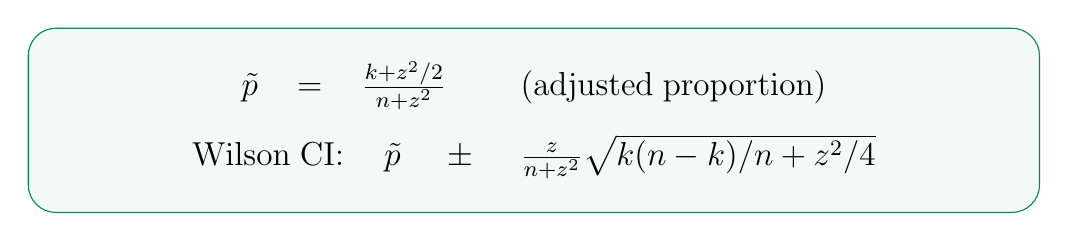
\begin{tikzpicture}
  \node[draw=paramgreen, fill=paramgreen!5, rounded corners=10pt, text width=12cm, align=center, inner sep=12pt] {
    {\large $\tilde{p} = \frac{k + z^2/2}{n + z^2}$ \qquad (adjusted proportion)}\\[8pt]
    {\large Wilson CI: $\;\tilde{p} \;\pm\; \frac{z}{n + z^2}\sqrt{k(n-k)/n + z^2/4}$}
  };
\end{tikzpicture}
\end{center}

\pause
\vspace{0.2cm}
\textbf{Intuition:} For 95\% CI ($z = 1.96 \approx 2$), Wilson acts like adding 2 successes and 2 failures:
$$\tilde{p} \approx \frac{k + 2}{n + 4}$$

\pause
\vspace{0.15cm}
\begin{center}
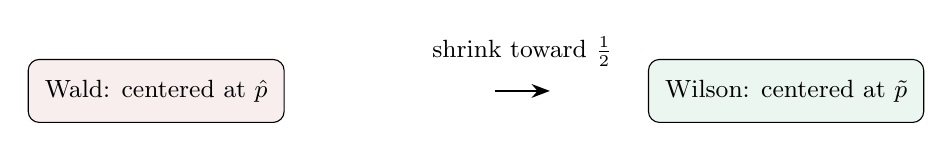
\begin{tikzpicture}[
  cbox/.style={draw, rounded corners=4pt, minimum height=0.8cm, align=center, font=\small, inner sep=6pt}
]
  \node[cbox, fill=warnred!8] at (-4, 0) {Wald: centered at $\hat{p}$};
  \node[cbox, fill=paramgreen!8] at (4, 0) {Wilson: centered at $\tilde{p}$};
  \draw[-{Stealth}, thick] (0.3, 0) -- (1, 0);
  \node[font=\small] at (0.65, 0.5) {shrink toward $\frac{1}{2}$};
\end{tikzpicture}
\end{center}

\vspace{0.1cm}
\centering\footnotesize
Wilson is the default in many statistics packages. Wald is mostly for teaching.
\end{frame}

\begin{frame}
\frametitle{Sample Size Planning}

\small
\textbf{Question:} How many voters must I survey for a $\pm 3\%$ margin of error at 95\% confidence?

\pause
\vspace{0.15cm}
\textbf{Start with the margin of error formula:}
$$\text{ME} = z_{\alpha/2} \cdot \sqrt{\frac{p(1-p)}{n}} \leq 0.03$$

\pause
\textbf{Solve for $n$} (use worst case $p = 0.5$):
$$n \geq \left(\frac{z_{\alpha/2}}{{\text{ME}}}\right)^2 \cdot p(1-p) = \left(\frac{1.96}{0.03}\right)^2 \cdot 0.25 = \textcolor{popblue}{1{,}068}$$

\pause
\vspace{0.15cm}
\begin{center}
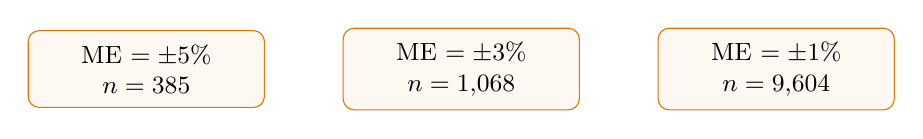
\begin{tikzpicture}[
  nbox/.style={draw=orange1, fill=orange1!5, rounded corners=4pt, minimum width=3cm, minimum height=0.8cm, align=center, font=\small, inner sep=5pt}
]
  \node[nbox] at (-4, 0) {ME $= \pm 5\%$\\$n = 385$};
  \node[nbox] at (0, 0) {ME $= \pm 3\%$\\$n = 1{,}068$};
  \node[nbox] at (4, 0) {ME $= \pm 1\%$\\$n = 9{,}604$};
\end{tikzpicture}
\end{center}

\vspace{0.1cm}
\centering\small The $\sqrt{n}$ law again: 10$\times$ more precision requires 100$\times$ more data.
\end{frame}

% ============================================================
\section{Beyond Wald: Other Intervals}

\begin{frame}
\begin{center}
  \vspace{2cm}
  {\Huge\bfseries\textcolor{popblue}{Beyond Wald}}

  \vspace{0.8cm}
  {\large $t$-intervals, likelihood intervals, and the Bayesian alternative}
\end{center}
\end{frame}

\begin{frame}
\frametitle{The $t$-Interval: When $\sigma$ Is Unknown}

\small
When $\sigma$ is unknown and estimated by $S$, use the $t$-distribution instead of $z$:

\pause
\vspace{0.05cm}
\begin{center}
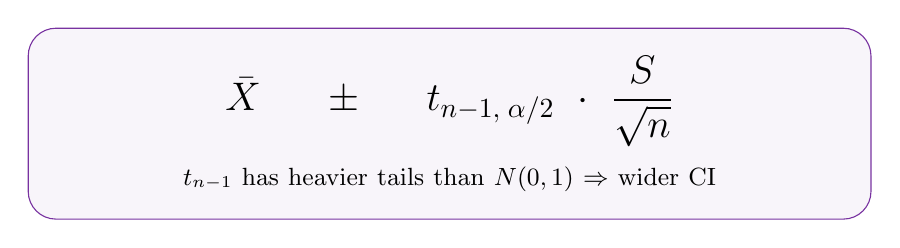
\begin{tikzpicture}
  \node[draw=violet1, fill=violet1!5, rounded corners=10pt, text width=10cm, align=center, inner sep=10pt] {
    {\Large $\bar{X} \;\pm\; t_{n-1,\;\alpha/2} \cdot \dfrac{S}{\sqrt{n}}$}\\[6pt]
    \small $t_{n-1}$ has heavier tails than $N(0,1)$ $\Rightarrow$ wider CI
  };
\end{tikzpicture}
\end{center}

\pause
\vspace{-0.05cm}
\begin{center}
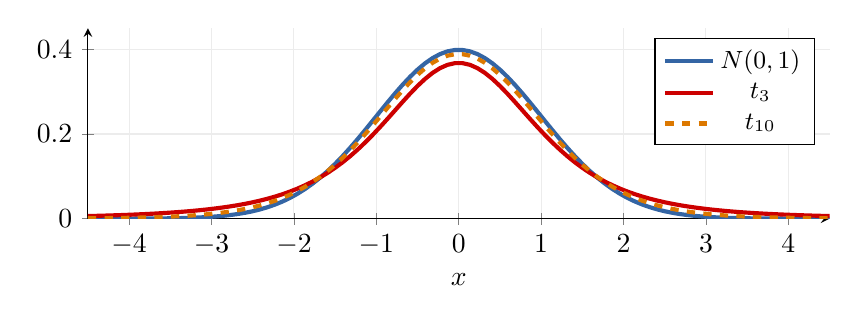
\begin{tikzpicture}
  \begin{axis}[
    width=11cm, height=4cm,
    xlabel={$x$},
    xmin=-4.5, xmax=4.5,
    ymin=0, ymax=0.45,
    axis lines=left,
    legend style={at={(0.98,0.95)}, anchor=north east, font=\small},
    grid=major, grid style={gray!15},
    every axis plot/.append style={line width=1.5pt, samples=100}
  ]
    \addplot[popblue, domain=-4.5:4.5] {exp(-x^2/2)/sqrt(2*pi)};
    \addlegendentry{$N(0,1)$}

    \addplot[sampred, domain=-4.5:4.5] {(1+x^2/3)^(-2) * 0.368};
    \addlegendentry{$t_3$}

    \addplot[orange1, dashed, domain=-4.5:4.5] {(1+x^2/10)^(-5.5) * 0.389};
    \addlegendentry{$t_{10}$}
  \end{axis}
\end{tikzpicture}
\end{center}

\vspace{-0.2cm}
\centering\footnotesize As $n \to \infty$: $t_{n-1} \to N(0,1)$. For $n \geq 30$, the difference is negligible.
\end{frame}

\begin{frame}
\frametitle{CI for Any MLE: The General Recipe}

\small
From Lecture~5: $\;\hat\theta_{\text{MLE}} \dot{\sim} N\!\left(\theta, \frac{1}{n \cdot I(\theta)}\right)$

\pause
\vspace{0.05cm}
\textbf{General Wald CI for the MLE:}
\begin{center}
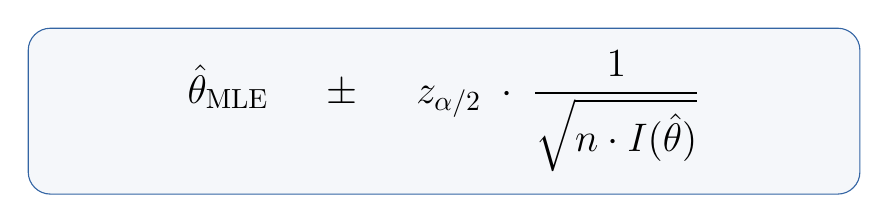
\begin{tikzpicture}
  \node[draw=popblue, fill=popblue!5, rounded corners=8pt, text width=10cm, align=center, inner sep=8pt] {
    {\Large $\hat\theta_{\text{MLE}} \;\pm\; z_{\alpha/2} \cdot \dfrac{1}{\sqrt{n \cdot I(\hat\theta)}}$}
  };
\end{tikzpicture}
\end{center}

\pause
\vspace{-0.05cm}
\textbf{Example: Poisson $\lambda$.} \; Fisher info: $I(\lambda) = 1/\lambda$. \; MLE: $\hat\lambda = \bar{X}$.
\vspace{-0.1cm}
$$\text{SE} = \frac{1}{\sqrt{n/\hat\lambda}} = \sqrt{\frac{\hat\lambda}{n}} \qquad \text{95\% CI: } \hat\lambda \pm 1.96\sqrt{\frac{\hat\lambda}{n}}$$

\vspace{-0.2cm}
\pause
\textbf{Concrete:} $n = 50$ earthquakes/year, $\hat\lambda = 3.2$. \;
$\text{SE} = \sqrt{3.2/50} = 0.253$. \; CI: $[2.70,\; 3.70]$.
\end{frame}

\begin{frame}
\frametitle{Confidence Intervals vs Credible Intervals}

\begin{center}
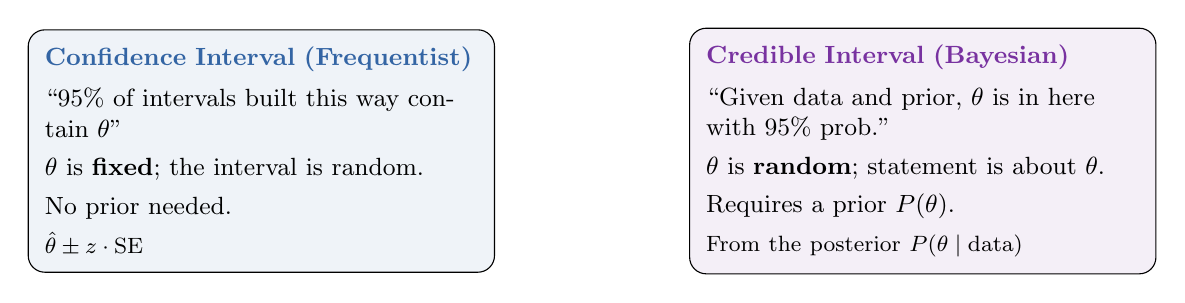
\begin{tikzpicture}[
  cbox/.style={draw, rounded corners=6pt, minimum height=3cm, text width=5.5cm, align=left, inner sep=6pt, font=\small}
]
  \node[cbox, fill=popblue!8] at (-4.2, 0) {
    \textbf{\textcolor{popblue}{Confidence Interval (Frequentist)}}\\[4pt]
    ``95\% of intervals built this way contain $\theta$''\\[3pt]
    $\theta$ is \textbf{fixed}; the interval is random.\\[3pt]
    No prior needed.\\[3pt]
    \footnotesize $\hat\theta \pm z \cdot \text{SE}$
  };

  \pause
  \node[cbox, fill=violet1!8] at (4.2, 0) {
    \textbf{\textcolor{violet1}{Credible Interval (Bayesian)}}\\[4pt]
    ``Given data and prior, $\theta$ is in here with 95\% prob.''\\[3pt]
    $\theta$ is \textbf{random}; statement is about $\theta$.\\[3pt]
    Requires a prior $P(\theta)$.\\[3pt]
    \footnotesize From the posterior $P(\theta \mid \text{data})$
  };
\end{tikzpicture}
\end{center}

\pause
\vspace{0.1cm}
\begin{center}
\fcolorbox{orange1}{orange1!5}{\parbox{10cm}{\centering\small
  With large $n$, they often give nearly identical intervals.\\
  The philosophical difference matters most with small $n$ or strong priors.\\[2pt]
  Neither is ``wrong'' --- they answer \textbf{different questions}.
}}
\end{center}
\end{frame}

\begin{frame}
\frametitle{The Delta Method: CIs for Transformations}

\small
\textbf{Problem:} You have a CI for $\theta$, but you want a CI for $g(\theta)$.

\pause
\vspace{0.15cm}
\textbf{Delta method:} If $\hat\theta \dot{\sim} N(\theta, \sigma^2_{\hat\theta})$, then for smooth $g$:
\begin{center}

\begin{tikzpicture}
  \node[draw=popblue, fill=popblue!5, rounded corners=8pt, text width=10cm, align=center, inner sep=10pt] {
    {\large $g(\hat\theta) \;\dot{\sim}\; N\!\bigl(g(\theta),\; [g'(\theta)]^2 \cdot \sigma^2_{\hat\theta}\bigr)$}\\[8pt]
    \small SE of $g(\hat\theta)$ $\;\approx\;$ $|g'(\hat\theta)| \cdot$ SE of $\hat\theta$
  };
\end{tikzpicture}
\end{center}

\pause
\vspace{0.15cm}
\textbf{Example: Odds ratio.} From $\hat{p}$, compute $\hat{\text{OR}} = \hat{p}/(1-\hat{p})$.
\begin{itemize}\setlength{\itemsep}{2pt}
  \item $g(p) = p/(1-p)$, \; $g'(p) = 1/(1-p)^2$
  \item $\text{SE}(\hat{\text{OR}}) \approx \frac{1}{(1-\hat{p})^2} \cdot \sqrt{\frac{\hat{p}(1-\hat{p})}{n}} = \frac{\sqrt{\hat{p}}}{(1-\hat{p})^{3/2}\sqrt{n}}$
\end{itemize}

\pause
\vspace{0.1cm}
\centering\footnotesize
\textbf{Tip:} Often easier to build CI on the log scale, then exponentiate the endpoints.\\
This gives asymmetric CIs, which are usually more appropriate for ratios.
\end{frame}

% ============================================================
\section{Summary}

\begin{frame}
\frametitle{Summary: From Point to Interval}
\begin{center}
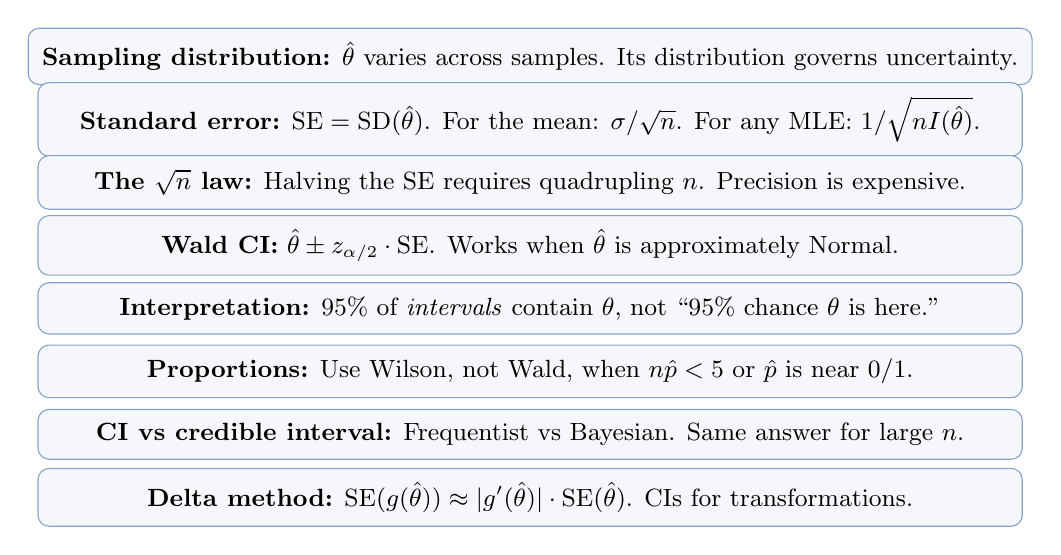
\begin{tikzpicture}[
  sbox/.style={draw=popblue!60, fill=popblue!5, rounded corners=4pt, minimum width=12.5cm, minimum height=0.5cm, align=left, inner sep=5pt, font=\small}
]
  \node[sbox] at (0, 2.8) {\textbf{Sampling distribution:} $\hat\theta$ varies across samples. Its distribution governs uncertainty.};
  \node[sbox] at (0, 2.0) {\textbf{Standard error:} $\text{SE} = \text{SD}(\hat\theta)$. For the mean: $\sigma/\sqrt{n}$. For any MLE: $1/\sqrt{nI(\hat\theta)}$.};
  \node[sbox] at (0, 1.2) {\textbf{The $\sqrt{n}$ law:} Halving the SE requires quadrupling $n$. Precision is expensive.};
  \node[sbox] at (0, 0.4) {\textbf{Wald CI:} $\hat\theta \pm z_{\alpha/2} \cdot \text{SE}$. Works when $\hat\theta$ is approximately Normal.};
  \node[sbox] at (0, -0.4) {\textbf{Interpretation:} 95\% of \textit{intervals} contain $\theta$, not ``95\% chance $\theta$ is here.''};
  \node[sbox] at (0, -1.2) {\textbf{Proportions:} Use Wilson, not Wald, when $n\hat{p} < 5$ or $\hat{p}$ is near 0/1.};
  \node[sbox] at (0, -2.0) {\textbf{CI vs credible interval:} Frequentist vs Bayesian. Same answer for large $n$.};
  \node[sbox] at (0, -2.8) {\textbf{Delta method:} $\text{SE}(g(\hat\theta)) \approx |g'(\hat\theta)| \cdot \text{SE}(\hat\theta)$. CIs for transformations.};
\end{tikzpicture}
\end{center}
\end{frame}

% ============================================================
\section{Practical}

\begin{frame}
\frametitle{Practical: Building Confidence Intervals}
\begin{center}
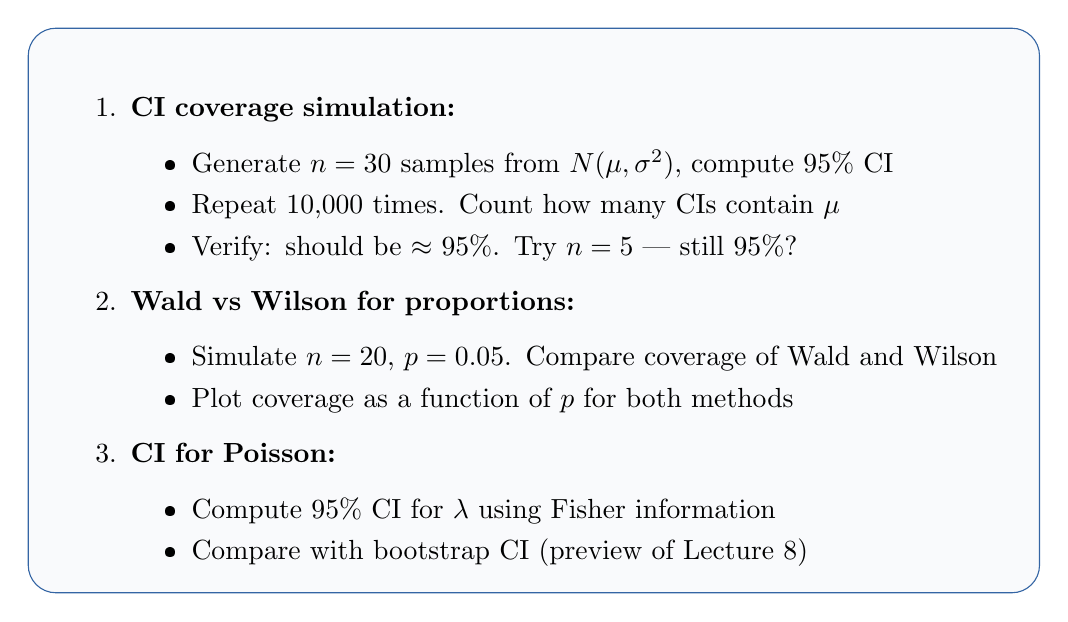
\begin{tikzpicture}
  \node[draw=popblue, fill=popblue!3, rounded corners=10pt, text width=12cm, align=left, inner sep=12pt] {
    \begin{enumerate}\setlength{\itemsep}{4pt}
      \item \textbf{CI coverage simulation:}
        \begin{itemize}\setlength{\itemsep}{1pt}
          \item Generate $n = 30$ samples from $N(\mu, \sigma^2)$, compute 95\% CI
          \item Repeat 10{,}000 times. Count how many CIs contain $\mu$
          \item Verify: should be $\approx$ 95\%. Try $n = 5$ --- still 95\%?
        \end{itemize}
      \item \textbf{Wald vs Wilson for proportions:}
        \begin{itemize}\setlength{\itemsep}{1pt}
          \item Simulate $n = 20$, $p = 0.05$. Compare coverage of Wald and Wilson
          \item Plot coverage as a function of $p$ for both methods
        \end{itemize}
      \item \textbf{CI for Poisson:}
        \begin{itemize}\setlength{\itemsep}{1pt}
          \item Compute 95\% CI for $\lambda$ using Fisher information
          \item Compare with bootstrap CI (preview of Lecture~8)
        \end{itemize}
    \end{enumerate}
  };
\end{tikzpicture}
\end{center}
\end{frame}

\begin{frame}
\frametitle{Homework}
\begin{enumerate}
  \item A factory tests $n = 100$ lightbulbs: $\bar{X} = 1{,}150$ hours, $S = 200$ hours.\\
    Construct 90\%, 95\%, and 99\% CIs for the true mean. Which is widest? Why?

  \vspace{0.15cm}
  \item A poll surveys $n = 500$ voters: 265 support candidate A ($\hat{p} = 0.53$).\\
    (a) Compute the Wald 95\% CI. Can we declare A is leading?\\
    (b) How many voters do we need for a $\pm 2\%$ margin of error?

  \vspace{0.15cm}
  \item For $X_1, \ldots, X_n \sim \text{Exp}(\lambda)$, the MLE is $\hat\lambda = 1/\bar{X}$.\\
    (a) Derive the SE using Fisher information ($I(\lambda) = 1/\lambda^2$).\\
    (b) Use the delta method to find a CI for the mean $\mu = 1/\lambda$.\\
    (c) Compare with a direct CI for $\mu$ using $\text{SE}(\bar{X}) = \bar{X}/\sqrt{n}$.

  \vspace{0.15cm}
  \item Simulate 1{,}000 Wald 95\% CIs for a proportion with $n = 15$, $p = 0.02$.\\
    What fraction contain $p$? Repeat with Wilson. Which is closer to 95\%?
\end{enumerate}
\end{frame}

\begin{frame}
\frametitle{Recommended Visualizations \& Resources}

\small
\begin{center}
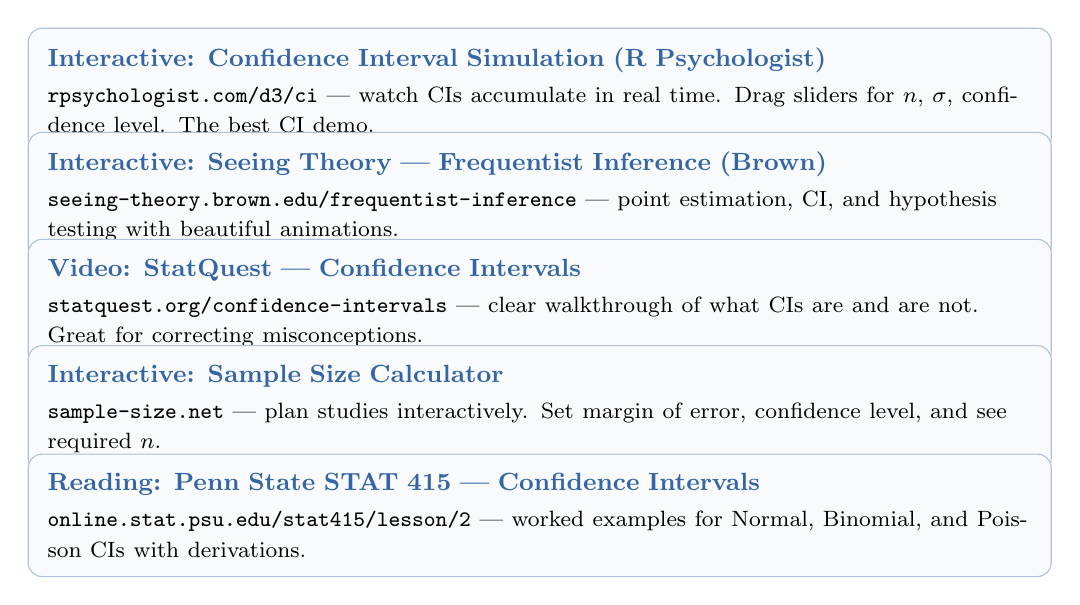
\begin{tikzpicture}[
  rbox/.style={draw=popblue!40, fill=popblue!3, rounded corners=5pt, text width=12.5cm, align=left, inner sep=7pt, font=\small}
]
  \node[rbox] at (0, 2.7) {
    \textbf{\textcolor{popblue}{Interactive: Confidence Interval Simulation (R Psychologist)}}\\[2pt]
    \footnotesize\texttt{rpsychologist.com/d3/ci} --- watch CIs accumulate in real time. Drag sliders for $n$, $\sigma$, confidence level. The best CI demo.
  };
  \node[rbox] at (0, 1.35) {
    \textbf{\textcolor{popblue}{Interactive: Seeing Theory --- Frequentist Inference (Brown)}}\\[2pt]
    \footnotesize\texttt{seeing-theory.brown.edu/frequentist-inference} --- point estimation, CI, and hypothesis testing with beautiful animations.
  };
  \node[rbox] at (0, 0.0) {
    \textbf{\textcolor{popblue}{Video: StatQuest --- Confidence Intervals}}\\[2pt]
    \footnotesize\texttt{statquest.org/confidence-intervals} --- clear walkthrough of what CIs are and are not. Great for correcting misconceptions.
  };
  \node[rbox] at (0, -1.35) {
    \textbf{\textcolor{popblue}{Interactive: Sample Size Calculator}}\\[2pt]
    \footnotesize\texttt{sample-size.net} --- plan studies interactively. Set margin of error, confidence level, and see required $n$.
  };
  \node[rbox] at (0, -2.7) {
    \textbf{\textcolor{popblue}{Reading: Penn State STAT 415 --- Confidence Intervals}}\\[2pt]
    \footnotesize\texttt{online.stat.psu.edu/stat415/lesson/2} --- worked examples for Normal, Binomial, and Poisson CIs with derivations.
  };
\end{tikzpicture}
\end{center}
\end{frame}

\begin{frame}
\begin{center}
  {\Huge\bfseries\textcolor{popblue}{Questions?}}

  \vspace{1cm}

  {\large Next: Lecture~8 --- Bootstrap and resampling methods}
\end{center}
\end{frame}

\end{document}
